\documentclass[a4paper,11pt,exos]{nsi} 
\usepackage{pifont}
\usepackage{fontawesome5}

\pagestyle{empty}



\begin{document}

\classe{\premiere spé}
\titre{Corrigé de l'évaluation 1 - Sujet A}
\maketitle


%\vspace{.5cm}
\exo{}
\textcolor{UGLiBlue}{On considère la fonction $f$ définie sur $\R$ par $\quad f(x)=-\dfrac{1}{2}(x+1)^2+5$.}

\begin{enumerate}%[label=\textbullet]
	\item 	\textcolor{UGLiBlue}{Compléter le tableau de variation de $f$ sur $\R$ :}
	\begin{center}
		\begin{tikzpicture}
			\tkzTabInit[lgt=3.5,espcl=3]
			{$x$ /.7 ,Variations de $f$ /2.5}
			{$-\infty$,$-1$,$+\infty$}
			\tkzTabVar{-/,+/$5$,-/}
		\end{tikzpicture}
	\end{center}
	\item 	\textcolor{UGLiBlue}{Calculer $f(1)$ et $f(3)$.}
	\begin{multicols}{2}
        \begin{tabbing}
            $f(1)$  \=$=-\dfrac{1}{2}\times (1+1)^2+5$\\[.5em]
                \>$=-\dfrac{1}{2}\times 2^2+5$\\[.5em]
                \>$=-\dfrac{1}{2}\times 4+5$\\
                \>$=-2+5$\\
                \>$=3$
        \end{tabbing}
        \begin{tabbing}
            $f(3)$  \=$=-\dfrac{1}{2}\times (3+1)^2+5$\\[.5em]
                \>$=-\dfrac{1}{2}\times 4^2+5$\\[.5em]
                \>$=-\dfrac{1}{2}\times 16+5$\\
                \>$=-8+5$\\
                \>$=-3$
        \end{tabbing}
    \end{multicols}
	\item 	
	\begin{minipage}{8cm}
		\textcolor{UGLiBlue}{Tracer la courbe représentative de $f$ dans le repère ci-contre.\\
		Indiquer les points utilisés.}
	\end{minipage}
	\begin{minipage}{8.7cm}
		\begin{center}
			\def\xmin{-6} \def\ymin{-5}\def\xmax{6}\def\ymax{7}
			\begin{tikzpicture}[scale=.6]
				\clip (\xmin,\ymin) rectangle (\xmax,\ymax);
				\draw[fill = white] (\xmin,\ymin) rectangle (\xmax,\ymax);
				\repereal{\xmin}{\ymin}{\xmax}{\ymax}
                \draw[thick,domain=\xmin:\xmax,smooth,variable=\x] plot ({\x},{-.5*(\x+1)^2+5});
                \draw (-1,5) \ball (1,3) \ball (3,-3)\ball (-3,3)\ball (-5,-3)\ball;
                \draw[UGLiRed] (-1,\ymax)--(-1,\ymin);
			\end{tikzpicture}
		\end{center}
	\end{minipage}
	
\end{enumerate}

\newpage
\exo{}
\begin{enumerate}
    \item \textcolor{UGLiBlue}{On définit la fonction $f$ sur $\R$ par $\quad f(x)=3(x-2)^2-5$.}
    \begin{multicols}{2}
        \begin{enumalph}
        \item \textcolor{UGLiBlue}{Donner la forme développée de $f$.}
        \begin{tabbing}
            $f(x)$  \=$=3\left(x^2-2\times x\times 2+2^2\right)-5$\\
            \>  $=3\left(x^2-4x+4\right)-5$\\
            \>  $=3x^2-12x+12-5$\\
            \>  $=3x^2-12x+7$
        \end{tabbing}
        \item \textcolor{UGLiBlue}{Tracer l'allure de la courbe représentative de $f$ en précisant les points remarquables.}\\
        \vfill\columnbreak
        \def\xmin{-1} \def\ymin{-6}\def\xmax{5}\def\ymax{8}
			\begin{tikzpicture}[yscale=.5]
				\clip (\xmin,\ymin) rectangle (\xmax,\ymax);
				\draw[fill = white] (\xmin,\ymin) rectangle (\xmax,\ymax);
				\repereal{\xmin}{\ymin}{\xmax}{\ymax}
                \draw[thick,domain=\xmin:\xmax,smooth,variable=\x] plot ({\x},{3*(\x-2)^2-5});
                \draw (2,-5) \ball (0,7) \ball ;
                %\draw[UGLiRed] (-1,\ymax)--(-1,\ymin);
			\end{tikzpicture}
    \end{enumalph}
    \end{multicols}
   
        
   
    \item \textcolor{UGLiBlue}{On définit la fonction $g$ sur $\R$ par $\quad g(x)=-\dfrac{1}{2}(x-2)(x+3)$.}
    \begin{multicols}{2}
        \begin{enumalph}
            \item \textcolor{UGLiBlue}{Donner la forme développée de $g$.}
            \begin{tabbing}
                $g(x)$  \=$=-\dfrac{1}{2}\left(x^2+3x-2x-6\right)$\\[.5em]
                \>  $=-\dfrac{1}{2}\left(x^2+x-6\right)$\\[.5em]
                \>  $=-\dfrac{1}{2}x^2-\dfrac{1}{2}x+3$
            \end{tabbing}
            \item \textcolor{UGLiBlue}{Tracer l'allure de la courbe représentative de $g$ en précisant les points remarquables.}
            \vfill\columnbreak
        \def\xmin{-5} \def\ymin{-3}\def\xmax{5}\def\ymax{5}
			\begin{tikzpicture}[scale=.6]
				\clip (\xmin,\ymin) rectangle (\xmax,\ymax);
				\draw[fill = white] (\xmin,\ymin) rectangle (\xmax,\ymax);
				\repereal{\xmin}{\ymin}{\xmax}{\ymax}
                \draw[thick,domain=\xmin:\xmax,smooth,variable=\x] plot ({\x},{-.5*(\x-2)*(\x+3)});
                \draw (-3,0) \ball (2,0)\ball (0,3) \ball ;
                %\draw[UGLiRed] (-1,\ymax)--(-1,\ymin);
			\end{tikzpicture}
        \end{enumalph}
    \end{multicols}
    
    
\end{enumerate}


\begin{minipage}{9cm}
	\exo{}
	\textcolor{UGLiBlue}{Voici un carré de côté 10 auquel on a ôté deux carrés de côtés $x+1$ et $x+3$ \textbf{qui ne se chevauchent pas} pour 
	obtenir la forme dessinée
	en gris foncé.}
\end{minipage}
\begin{minipage}{8cm}
	\begin{center}
		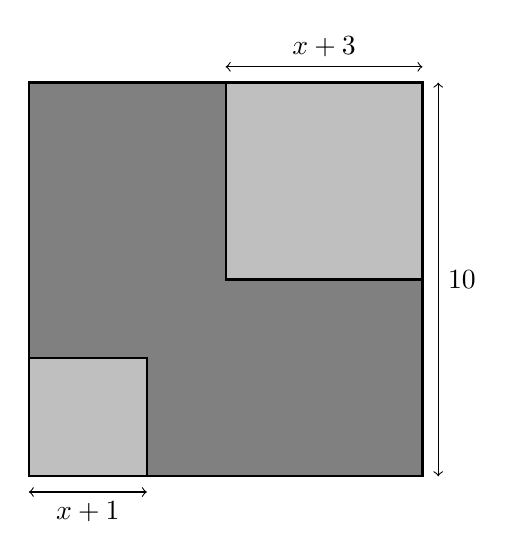
\begin{tikzpicture}[scale = .5]
			\draw[thick, fill = gray] (0,0)  rectangle (10,10);
			\draw[thick, fill = lightgray] (0,0)  rectangle (3,3);
			\draw[thick, fill = lightgray] (10,10)  rectangle (5,5);
			\draw[<->] (5,10.4) -- node[midway,above]{$x+3$} (10,10.4);
			\draw[<->] (10.4,0) -- node[midway,right]{10} (10.4,10);
			\draw[<->] (0,-.4) -- node[midway,below]{$x+1$} (3,-.4);
		\end{tikzpicture}
	\end{center}
\end{minipage}



\begin{enumerate}
	\item 	\textcolor{UGLiBlue}{Quelle est la valeur minimale que peut prendre la variable $x$ ? Sa valeur maximale ?\\
    En déduire l'intervalle dans lequel varie $x$.}\\[.5em]
	Les longueurs $\ x+1\ $ et $\ x+3\ $ doivent être positives. D'où $\quad x>-1$.\\
	Les carrés ne doivent pas se chevaucher donc $x+1+x+3$ doit être inférieur à $10$.
	\begin{tabbing}
		$x+1+x+3<10 \quad$	\= $\iff \quad 2x+4<10$\\
		\>	$\iff \quad 2x<6$\\
		\>	$\iff \quad x<3$
	\end{tabbing}
	Ainsi $\ x\in\oio{-1}{3}$.
	
	\item 	\textcolor{UGLiBlue}{Montrer que l'aire $A(x)$ de la figure gris foncé est : $A(x)=-2x^2-8x+90$.}\\[.5em]
	Soit $x\in\oio{-1}{3}$.
	\begin{tabbing}
		$A(x)$	\=$=10^2-(x+1)^2-(x+3)^2$\\
		\>	$=100-(x^2+2\times x\times 1+1^2)+(x^2+2\times x\times 3+3^2)$\\
		\>	$= 100-(x^2+2x+1)-(x^2+6x+9)$\\
		\>	$=100-x^2-2x-1-x^2-6x-9$\\
		\>	$=-2x^2-8x+90$
	\end{tabbing}

	
    \item \textcolor{UGLiBlue}{Donner la forme canonique de $A$.}\\[.5em]
	Soit $x\in\oio{-1}{3}$.
	\begin{tabbing}
		$A(x)$	\=$=-2x^2-8x+90$\\
		\>	$=-2\left[x^2+4x-45\right]$\\
		\>	$=-2\left[x^2+2\times x\times 2+2^2-2^2-45\right]$\\
		\>	$=-2\left[(x+2)^2-4-45\right]$\\
		\>	$=-2\left[(x+2)^2-49\right]$\\
		\>	$=-2(x+2)^2+98$
	\end{tabbing}

	
	\item 	\textcolor{UGLiBlue}{Peut-on faire en sorte que l'aire en gris foncé soit égale à 50 ?\\
	Si oui, pour quelle(s) valeur(s) de $x$ ?}\\[.5em]
	Soit $x\in\oio{-1}{3}$.
	\begin{tabbing}
		$A(x)=50\quad$	\=$\iff\quad -2(x+2)^2+98=50$\\
		\>	$\iff\quad -2(x+2)^2=-48$\\
		\>	$\iff\quad	(x+2)^2=24$\\
		\>	$\iff\quad	x+2=-\sqrt{24}\quad \text{ou} \quad x+2=\sqrt{24}$\\
		\>	$\iff\quad	x=-2-\sqrt{24}\quad \text{ou} \quad x=-2+\sqrt{24}$
	\end{tabbing}
	Or $\quad -2-\sqrt{24}<-2\quad$ donc $\quad -2-\sqrt{24} \notin \oio{-1}{3}$.\\
	Et $\quad 4<\sqrt{24}<5\quad$ donc $\quad 2<-2+\sqrt{24}<3\quad$ et ainsi $\quad -2+\sqrt{24} \in \oio{-1}{3}$.\\[.5em]
	L'aire en gris foncé ne peut être égale à $50$ que lorsque $x=-2+\sqrt{24}$.
\end{enumerate}

%\vspace*{.5cm}

\newpage


\dleft{10cm}{
\exo{}
\textcolor{UGLiBlue}{$f$ est la fonction polynôme du second degré représentée graphiquement par la parabole ci-contre.}\\

\textcolor{UGLiBlue}{Déterminer l'expression algébrique de $f$ à l'aide des trois points indiqués sur la parabole.}}
{
    \def\xmin{-6} \def\ymin{-6}\def\xmax{6}\def\ymax{6}
			\begin{tikzpicture}[scale=.5]
				\clip (\xmin,\ymin) rectangle (\xmax,\ymax);
				\draw[fill = white] (\xmin,\ymin) rectangle (\xmax,\ymax);
				\repereal{\xmin}{\ymin}{\xmax}{\ymax}
                \draw[UGLiRed, thick, domain=\xmin:\xmax,variable=\x] plot({\x},{1/3*(\x-4)*(\x+3)});		
                \draw (0,-4) \ball (4,0) \ball (-3,0) \ball;
			\end{tikzpicture}
}

\vspace*{.5cm}
On lit que la fonction $f$ a pour racines $-3$ et $4$.
\begin{tabbing}
	Il existe donc un réel non nul $a$ tel que, pour tout $x\in\R, \quad f(x)$	\=$=a\left(x-(-3)\right)(x-4)$\\
	\>	$=a(x+3)(x-4)$
\end{tabbing}
De plus la parabole coupe l'axe des ordonnées en $-4$ donc $f(0)=-4$.
\begin{tabbing}
	$f(0)=-4\quad$	\=	$\iff\quad a\times (0+3)\times (0-4)=-4$\\
	\>	$\iff\quad -12a=-4$\\
	\>	$\iff\quad	a=\dfrac{-4}{-12}$\\[.5em]
	\>	$\iff\quad	a=\dfrac{1}{3}$
\end{tabbing}
D'ou, pour tout $x\in\R, \quad f(x)=\dfrac{1}{3}(x+3)(x-4)$.

\setcounter{section}{0}
\newpage

%%%%%%%%%%%%%%%%%%%%%%%%%%%%%%%%%%%%%%%%%%%%%%%%%%%%%%%%%%%%%%%%%%%
\classe{\premiere spé}
\titre{Corrigé de l'évaluation 1 - Sujet B}
\maketitle


\exo{}
\textcolor{UGLiBlue}{On considère la fonction $f$ définie sur $\R$ par $\quad f(x)=\dfrac{1}{2}(x+2)^2-3$.}

\begin{enumerate}%[label=\textbullet]
	\item 	\textcolor{UGLiBlue}{Compléter le tableau de variation de $f$ sur $\R$ :}
	\begin{center}
		\begin{tikzpicture}
			\tkzTabInit[lgt=3.5,espcl=3]
			{$x$ /.7 ,Variations de $f$ /2.5}
			{$-\infty$,$-2$,$+\infty$}
			\tkzTabVar{+/,-/$-3$,+/}
		\end{tikzpicture}
	\end{center}
	\item 	\textcolor{UGLiBlue}{Calculer $f(0)$ et $f(2)$.}
	\begin{multicols}{2}
        \begin{tabbing}
            $f(0)$  \=$=\dfrac{1}{2}\times (0+2)^2-3$\\[.5em]
                \>$=\dfrac{1}{2}\times 2^2-3$\\[.5em]
                \>$=\dfrac{1}{2}\times 4-3$\\
                \>$=2-3$\\
                \>$=-1$
        \end{tabbing}
        \begin{tabbing}
            $f(2)$  \=$=\dfrac{1}{2}\times (2+2)^2-3$\\[.5em]
                \>$=\dfrac{1}{2}\times 4^2-3$\\[.5em]
                \>$=\dfrac{1}{2}\times 16-3$\\
                \>$=8-3$\\
                \>$=5$
        \end{tabbing}
    \end{multicols}
	\item 	
	\begin{minipage}{7.7cm}
		\textcolor{UGLiBlue}{Tracer la courbe représentative de $f$ dans le repère ci-contre.\\
        Indiquer les points utilisés.}
	\end{minipage}
	\begin{minipage}{8.7cm}
		\begin{center}
			\def\xmin{-7} \def\ymin{-5}\def\xmax{6}\def\ymax{7}
			\begin{tikzpicture}[scale=.6]
				\clip (\xmin,\ymin) rectangle (\xmax,\ymax);
				\draw[fill = white] (\xmin,\ymin) rectangle (\xmax,\ymax);
				\repereal{\xmin}{\ymin}{\xmax}{\ymax}	
				\draw[thick,domain=\xmin:\xmax,smooth,variable=\x] plot ({\x},{.5*(\x+2)^2-3});
                \draw (-2,-3) \ball (0,-1) \ball (2,5)\ball (-4,-1)\ball (-6,5)\ball;
                \draw[UGLiRed] (-2,\ymax)--(-2,\ymin);	
			\end{tikzpicture}
		\end{center}
	\end{minipage}
	
\end{enumerate}

\newpage
\exo{}
\begin{enumerate}
    \item \textcolor{UGLiBlue}{On définit la fonction $f$ sur $\R$ par $\quad f(x)=-2(x-3)^2+10$.}
    \begin{multicols}{2}
		\begin{enumalph}
			\item \textcolor{UGLiBlue}{Donner la forme développée de $f$.}
			\begin{tabbing}
				$f(x)$	\=$=-2\left(x^2-2\times x\times 3+3^2\right)+10$\\
				\>	$=-2\left(x^2-6x+9\right)+10$\\
				\>	$=-2x^2+12x-18+10$\\
				\>	$=-2x^2+12x-8$
			\end{tabbing}
			\item \textcolor{UGLiBlue}{Tracer l'allure de la courbe représentative de $f$ en précisant les points remarquables.}\\
			\vfill\columnbreak
        \def\xmin{-1} \def\ymin{-10}\def\xmax{7}\def\ymax{12}
			\begin{tikzpicture}[xscale=.7,yscale=.3]
				\clip (\xmin,\ymin) rectangle (\xmax,\ymax);
				\draw[fill = white] (\xmin,\ymin) rectangle (\xmax,\ymax);
				\repereal{\xmin}{\ymin}{\xmax}{\ymax}
                \draw[thick,domain=\xmin:\xmax,smooth,variable=\x] plot ({\x},{-2*(\x-3)^2+10});
                \draw (3,10) \ball (0,-8) \ball ;
                %\draw[UGLiRed] (-1,\ymax)--(-1,\ymin);
			\end{tikzpicture}
		\end{enumalph}
	\end{multicols}
    

    \item \textcolor{UGLiBlue}{On définit la fonction $g$ sur $\R$ par $\quad g(x)=\dfrac{1}{2}(x+2)(x-3)$.}
    \begin{multicols}{2}
		\begin{enumalph}
			\item \textcolor{UGLiBlue}{Donner la forme développée de $g$.}
			\begin{tabbing}
				$g(x)$	\=$=\dfrac{1}{2}\left(x^2-3x+2x-6\right)$\\[.5em]
				\>	$= \dfrac{1}{2}\left(x^2-x-6\right)$\\[.5em]
				\>	$= \dfrac{1}{2}x^2-\dfrac{1}{2}x-3$
			\end{tabbing}
			\item \textcolor{UGLiBlue}{Tracer l'allure de la courbe représentative de $g$ en précisant les points remarquables.}\\
			\vfill\columnbreak
        \def\xmin{-4} \def\ymin{-4}\def\xmax{5}\def\ymax{4}
			\begin{tikzpicture}[scale=.6]
				\clip (\xmin,\ymin) rectangle (\xmax,\ymax);
				\draw[fill = white] (\xmin,\ymin) rectangle (\xmax,\ymax);
				\repereal{\xmin}{\ymin}{\xmax}{\ymax}
                \draw[thick,domain=\xmin:\xmax,smooth,variable=\x] plot ({\x},{.5*(\x-3)*(\x+2)});
                \draw (-2,0) \ball (3,0)\ball (0,-3) \ball ;
                %\draw[UGLiRed] (-1,\ymax)--(-1,\ymin);
			\end{tikzpicture}
		\end{enumalph}
	\end{multicols}
    
    
\end{enumerate}


\begin{minipage}{9cm}
	\exo{}
	\textcolor{UGLiBlue}{Voici un carré de côté 8 auquel on a ôté deux carrés de côtés $x+1$ et $x+3$ \textbf{qui ne se chevauchent pas} pour 
	obtenir la forme dessinée
	en gris foncé.}
\end{minipage}
\begin{minipage}{8cm}
	\begin{center}
		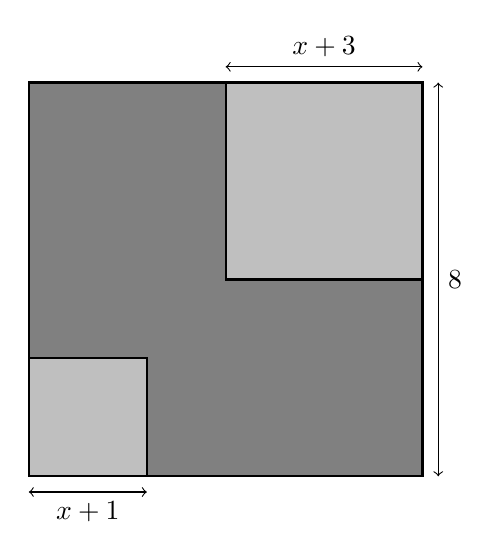
\begin{tikzpicture}[scale = .5]
			\draw[thick, fill = gray] (0,0)  rectangle (10,10);
			\draw[thick, fill = lightgray] (0,0)  rectangle (3,3);
			\draw[thick, fill = lightgray] (10,10)  rectangle (5,5);
			\draw[<->] (5,10.4) -- node[midway,above]{$x+3$} (10,10.4);
			\draw[<->] (10.4,0) -- node[midway,right]{8} (10.4,10);
			\draw[<->] (0,-.4) -- node[midway,below]{$x+1$} (3,-.4);
		\end{tikzpicture}
	\end{center}
\end{minipage}



\begin{enumerate}
	\item 	\textcolor{UGLiBlue}{Quelle est la valeur minimale que peut prendre la variable $x$ ? Sa valeur maximale ?\\
    En déduire l'intervalle dans lequel varie $x$.}\\[.5em]
	Les longueurs $\ x+1\ $ et $\ x+3\ $ doivent être positives. D'où $\quad x>-1$.\\
	Les carrés ne doivent pas se chevaucher donc $x+1+x+3$ doit être inférieur à $8$.
	\begin{tabbing}
		$x+1+x+3< \quad$	\= $\iff \quad 2x+4<8$\\
		\>	$\iff \quad 2x<4$\\
		\>	$\iff \quad x<2$
	\end{tabbing}
	Ainsi $\ x\in\oio{-1}{2}$.
	
	\item 	\textcolor{UGLiBlue}{Montrer que l'aire $A(x)$ de la figure gris foncé est : $A(x)=-2x^2-8x+54$.}\\[.5em]
	Soit $x\in\oio{-1}{2}$
	\begin{tabbing}
		$A(x)$	\=$=8^2-(x+1)^2-(x+3)^2$\\
		\>	$=64-(x^2+2\times x\times 1+1^2)+(x^2+2\times x\times 3+3^2)$\\
		\>	$= 64-(x^2+2x+1)-(x^2+6x+9)$\\
		\>	$=64-x^2-2x-1-x^2-6x-9$\\
		\>	$=-2x^2-8x+54$
	\end{tabbing}

   
    \item \textcolor{UGLiBlue}{Donner la forme canonique de $A$.}\\[.5em]
	Soit $x\in\oio{-1}{2}$
	\begin{tabbing}
		$A(x)$	\=$=-2x^2-8x+54$\\
		\>	$=-2\left[x^2+4x-27\right]$\\
		\>	$= -2\left[x^2+2\times x\times 2+2^2-2^2-27\right]$\\
		\>	$=-2\left[(x+2)^2-4-27\right]$\\
		\>	$=-2\left[(x+2)^2-31\right]$\\
		\>	$=-2(x+2)^2+62$
	\end{tabbing}

	
	\item 	\textcolor{UGLiBlue}{Peut-on faire en sorte que l'aire en gris foncé soit égale à 50 ?\\
	Si oui, pour quelle(s) valeur(s) de $x$ ?}\\[.5em]
	Soit $x\in\oio{-1}{2}$
	\begin{tabbing}
		$A(x)=50$	\=$\iff\quad -2(x+2)^2+62=50$\\
		\>	$\iff\quad -2(x+2)^2=-12$\\
		\>	$\iff\quad	(x+2)^2=6$\\
		\>	$\iff\quad	x+2=-\sqrt{6}\quad$ ou $\quad x+2=\sqrt{6}$\\
		\>	$\iff\quad	x=-2-\sqrt{6}\quad$ ou $\quad x=-2+\sqrt{6}$
	\end{tabbing}
	Or $\quad -2-\sqrt{6}<-2\quad$ donc $\quad -2-\sqrt{6}\notin\oio{-1}{2}$.\\
	Et $\quad 2<\sqrt{6}<3\quad$ donc $\quad 0<-2+\sqrt{6}<1\quad$ et ainsi $\quad -2+\sqrt{6}\in\oio{-1}{2}$.\\[.5em]
	L'aire en gris foncé ne peut être égale à $50$ que lorsque $x=-2+\sqrt{6}$.
\end{enumerate}

%\vspace*{.5cm}

\newpage


\dleft{10cm}{
\exo{}
\textcolor{UGLiBlue}{$f$ est la fonction polynôme du second degré représentée graphiquement par la parabole ci-contre.}\\

\textcolor{UGLiBlue}{Déterminer l'expression algébrique de $f$ à l'aide des trois points indiqués sur la parabole.}}
{
    \def\xmin{-4} \def\ymin{-5}\def\xmax{8}\def\ymax{7}
			\begin{tikzpicture}[scale=.5]
				\clip (\xmin,\ymin) rectangle (\xmax,\ymax);
				\draw[fill = white] (\xmin,\ymin) rectangle (\xmax,\ymax);
				\repereal{\xmin}{\ymin}{\xmax}{\ymax}
                \draw[UGLiRed, thick, domain=\xmin:\xmax,variable=\x] plot({\x},{-1/3*(\x-6)*(\x+2)});		
                \draw (0,4) \ball (6,0) \ball (-2,0) \ball;
			\end{tikzpicture}
}

\vspace*{.5cm}
On lit que la fonction $f$ a pour racines $-2$ et $6$.
\begin{tabbing}
	Il existe donc un réel non nul $a$ tel que, pour tout $x\in\R, \quad f(x)$	\=$=a\left(x-(-2)\right)(x-6)$\\
	\>	$=a(x+2)(x-6)$
\end{tabbing}
De plus la parabole coupe l'axe des ordonnées en $4$ donc $f(0)=4$.
\begin{tabbing}
	$f(0)=4\quad$	\=	$\iff\quad a\times (0+2)\times (0-6)=4$\\
	\>	$\iff\quad -12a=4$\\
	\>	$\iff\quad	a=-\dfrac{4}{12}$\\[.5em]
	\>	$\iff\quad	a=-\dfrac{1}{3}$
\end{tabbing}
D'ou, pour tout $x\in\R, \quad f(x)=-\dfrac{1}{3}(x+2)(x-6)$.
\end{document}